\documentclass[a4paper]{article}

\usepackage[margin=1.2in]{geometry}

\usepackage[T1]{fontenc}
\usepackage[francais]{babel}
\usepackage{fontspec}
\setmainfont{Droid Serif}
\setmonofont{Inconsolata}

\usepackage{url}
\usepackage{hyperref}

\usepackage{fancyhdr}
\pagestyle{fancy}

\usepackage{graphicx}

\usepackage{minted}

\definecolor{foreground}{RGB}{21,21,21}
\definecolor{background}{RGB}{242,245,227}
\definecolor{title}{RGB}{255,31,110}
\definecolor{gray}{RGB}{155,155,155}
\definecolor{toogyblue}{RGB}{87,102,181}

\newminted{csharp}{bgcolor=gray!25,fontsize=\normalsize,mathescape,linenos,frame=lines,framerule=0.3pt}

\newcommand{\tptitle}
    {\textbf{TP BDSP 13/14} $\bullet$ T'es triste $\bullet$ \textbf{GConfs}}

\fancyhf{}
\lhead{\textbf{\thepage}}
\rhead{\tptitle{}}
\lfoot{\tptitle{}}
\rfoot{\textbf{\thepage}}
\renewcommand{\headrulewidth}{0.4pt}
\renewcommand{\footrulewidth}{0.4pt}

\setcounter{tocdepth}{1}

% END STYLE

\title{T'es triste}

\author{
    GConfs
}

\date{15 novembre 2013}

\begin{document}
\color{foreground}

%
\begin{center}
    \fbox{
        \begin{minipage}[t]{6cm}
            \begin{center}
                \textbf{\huge T'es triste} \\
                \emph{\color{red} TP BDSP 13/14}
            \end{center}
        \end{minipage}
    }
\end{center}

\section*{Introduction}

Dans ce TP, vous allez devoir réaliser un tétris très simplifié : les pièces
sont de taille 3 (et non 4) et elles ne peuvent pas tourner. \\

\begin{center}
    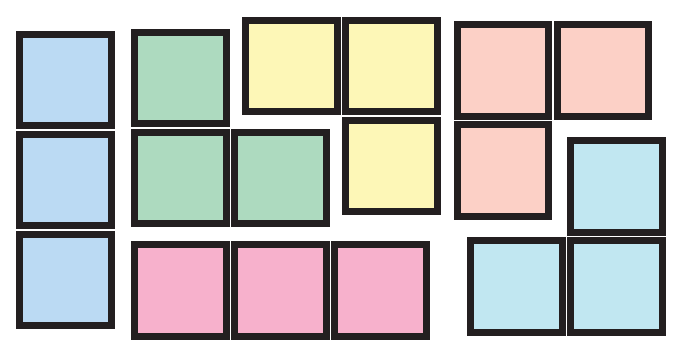
\includegraphics[scale=0.5]{img/pieces.eps}
\end{center}

Ce TP est fait pour être réalisé en équipe (2-4 membres) mais vous pouvez très
bien le faire tout seul, si vous en êtes capable (même si c'est moins marrant).
\\

\textbf{But du TP :} apprendre à utiliser \textbf{Git} à plusieurs et apprendre
les bases d'\textbf{XNA}.

\begin{center}\noindent\rule{12cm}{0.4pt}\end{center}

\tableofcontents

\begin{center}\noindent\rule{12cm}{0.4pt}\end{center}

\section{Création du dépôt Git et du projet XNA}

\noindent{\color{red} Si vous êtes bloqué à une étape, les assistants sont là pour vous
aider. Alors n'hésitez pas à leur demander.}

\begin{enumerate}
    \item Commencez par tous vous inscrire sur \url{https://bitbucket.org} ou
    \url{http://github.com} (mais tous les membres au même endroit sinon ça va
    pas le faire). \\
    Ces deux sites permettent à des développeurs d'héberger leurs dépôts Git, et ce
    gratuitement.\\
    \textbf{Attention} : GitHub ne permet pas de faire de dépôt privé
    de base; il faut un compte étudiant. Préférez BitBucket si vous n'êtes pas
    quelqu'un d'opensource.\\

    {\color{red} \textbf{Attention} : \\Les étapes \textbf{2} et \textbf{3}
    sont faites par une seule personne. Choisissez la. Les autres regardent et
    l'aident.}\\

    \item L'heureux élu se rend donc sur le site que vous avez choisi et créé un
    nouveau dépôt (en général y'a un gros bouton pour ça, vous allez y arriver). \\

    \item Cette même personne créé un nouveau projet XNA sur VS.
\end{enumerate}

\% \textbf{TODO}: Corwin doit rajouter des étapes pour l'extension Git de VS
À la fin, ils sont tous sensés avoir le nouveau projet sur leur VS. \\
Expliquer comment utiliser l'extension pour commit, push etc.

\section{Principe du jeu}

\begin{center}
    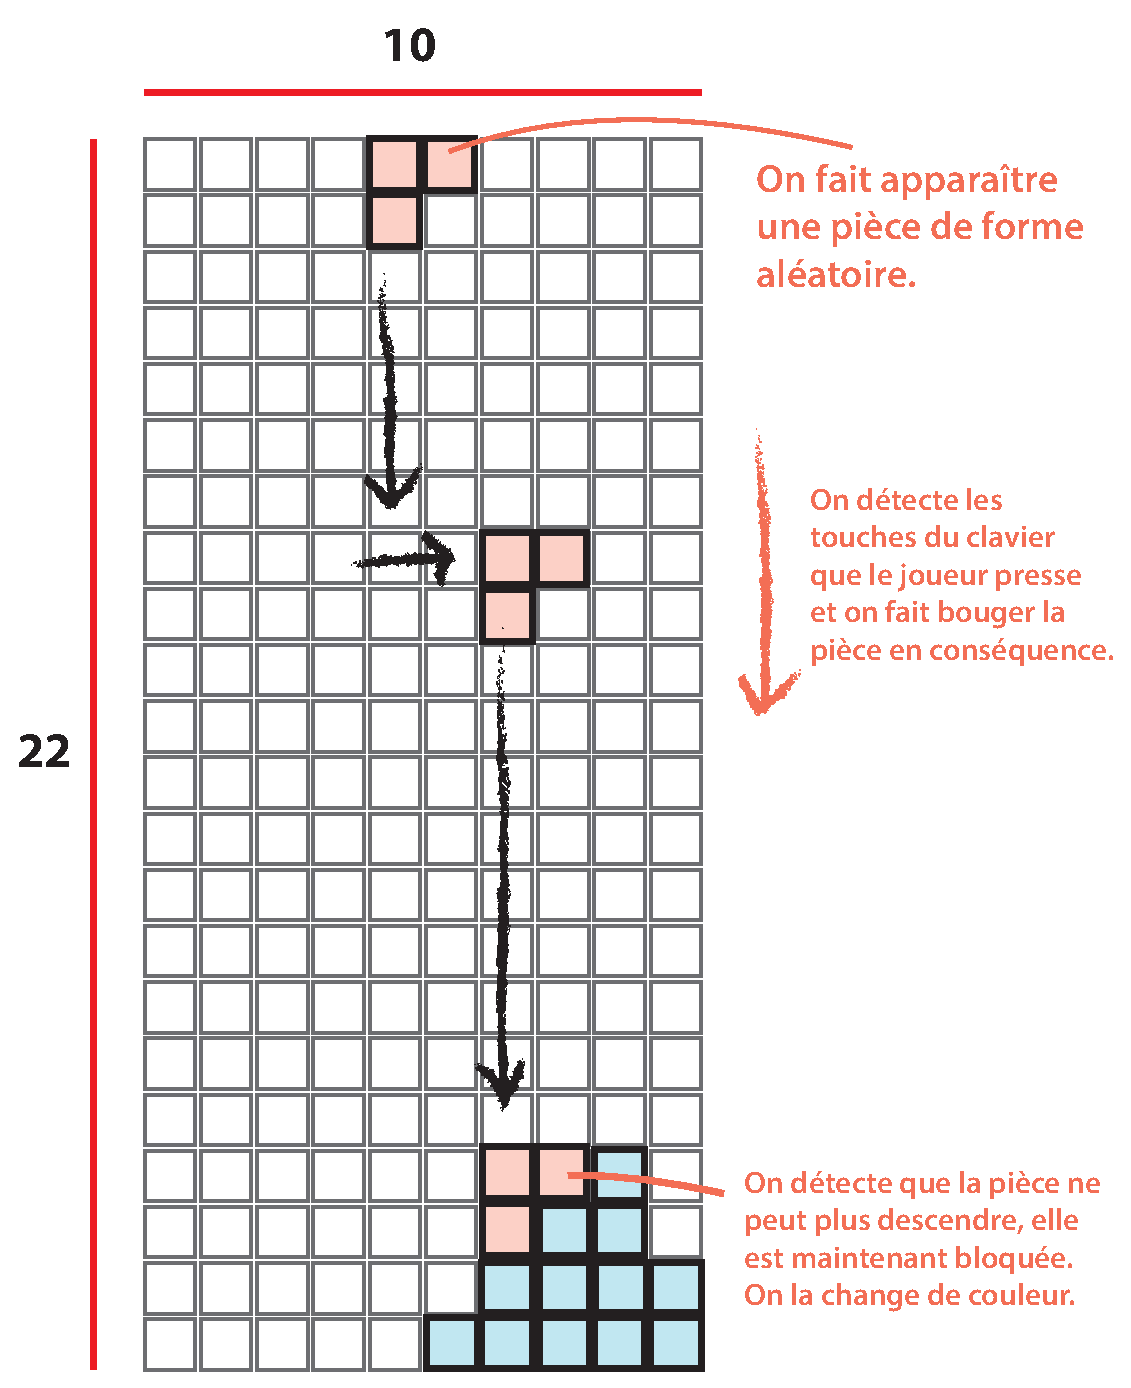
\includegraphics[scale=0.7]{img/game-explanation.eps} 
\end{center}

\noindent\textbf{Remarque} : ce processus tourne en boucle puisque quand une
pièce devient bloquée, on en fait apparaître une nouvelle qui subira le même
sort que la précédente.

\newpage
\section{Liste des fonctionnalités à implémenter}

\begin{enumerate}
    \item TexturesManager : charger les textures à dessiner
    \item Plateau de jeu (map sur laquelle les pièces se déplaceront)
    \item Pièce (composée de 3 cases)
        \begin{enumerate}
            \item Génération d'une pièce aléatoire
            \item Déplacement
        \end{enumerate}
    \item Boucle de jeu principale
        \begin{enumerate}
            \item Initialisation du jeu (dans la fonction du même nom)
            \item Détection du GameOver
            \item Update() : Détection de l'input du joueur (touches clavier)
            \item Draw()
        \end{enumerate}
\end{enumerate}

\begin{center}
    {\large\color{red} Pour vous aider, la partie \textbf{5} vous explique
    comment implémenter chaque fonctionnalité. Vous n'êtes pas obligés de vous
    en servir. Si vous voulez un peu plus de challenge vous pouvez proposer
    votre propre implémentation. :) Vous êtes libres.}
\end{center}

\section{Les images du jeu sont fournies !}

Pour les téléchargez, rendez vous ici : \url{http://too.gy/bdsp/tp.zip}. \\

\begin{itemize}
    \item[\textbf{GameBackground.png}]: image de fond du jeu, avec le plateau. On affichera
        les autres élements (comme les pièces) par dessus. \\

    \item[\textbf{GameOver.png}]: image à moitié transparente. On l'affichera par dessus
        toutes les autres quand la partie sera terminée. \\

    \item[\textbf{Piece.jpg}]: image d'une pièce \\

    \item[\textbf{PieceBlocked.jpg}] : image d'une pièce bloquée
\end{itemize}

\section{Comment implémenter tout ça}

\subsection{TexturesManager : chargement des textures}

On va commencer par charger nos textures dans notre jeu. Comme ça ce sera fait
et on y aura accès par la suite. \\

Pour charger des images et les mettres sous forme de textures, XNA se sert d'un
objet appelé le 'ContentManager' : \\

\begin{csharpcode}
// Vous remarquerez qu'il n'y a pas l'extension sur le nom du fichier
Texture2D MaTexture = content.Load<SpriteFont>("MonFicher");
\end{csharpcode}

\vspace{0.2cm}

Ce qu'on va faire, c'est créer une sorte de 'service', une classe statique qui
va contenir nos textures, à laquelle on aura accès depuis n'importe quelle
classe de notre solution (projet). \\

\begin{csharpcode*}{label=TexturesManager.cs}
// ATTENTION au mot clef 'static'
public static class TexturesManager
{
    public static Texture2D GameBackground,
                            GameOver,
                            Piece,
                            PieceBlocked;

    public static void LoadContent(ContentManager content)
    {
        // TODO: Charger les 4 textures
    }
}
\end{csharpcode*}

\vspace{0.2cm}

Il faut appeler la fonction LoadContent de notre TexturesManager depuis la
classe principale 'Game1', dans sa propre fonction LoadContent : \\

\begin{csharpcode*}{label=Game1.cs}
protected override void LoadContent()
{
    IsMouseVisible = true;
    spriteBatch = new SpriteBatch(GraphicsDevice);

    TexturesManager.LoadContent(Content);
}
\end{csharpcode*}

\vspace{0.2cm}
On peut maintenant accéder à nos 4 textures depuis n'importe quelle classe de
la façon suivante : \\

\begin{csharpcode}
TexturesManager.NomDeLaTexture;
\end{csharpcode}

\subsection{Plateau de jeu}

\subsubsection{Principe}

Notre plateau de jeu est composé de \textbf{10} cases sur la coordonnée $x$ de
XNA et de \textbf{22} cases sur sa coordonnée $y$. (voir schéma 'Principe du jeu')\\
Pour chaque case on a envie de savoir si la case est occupée par soit :

\begin{itemize}
    \item une case vide
    \item un bloc d'une pièce bloquée (une pièce est constituée de 3 blocs)
    \item un bloc d'une pièce non-bloquée
\end{itemize}

(on différencie pièce bloquée et non-bloquée car on veut les afficher
différemment). \\

Le plus simple c'est de représenter les cases notre plateau par un tableau de
bytes : \\

\begin{csharpcode*}{label=Plate.cs}
public class Plate
{
    public byte[,] Cells { get; set; }
}
\end{csharpcode*}

\vspace{0.2cm}

Pour accéder à une case de notre plateau, il suffit alors de faire : \\

\begin{csharpcode}
Plate p = new Plate();

byte b = p.Cells[0,0]; // récupère la case tout en haut à gauche
\end{csharpcode}

\vspace{0.2cm}

Pour parcourir l'ensemble de nos cases, il suffit de faire : \\

\begin{csharpcode}
for (int x = 0; x < 10; x++)
{
    for (int y = 0; y < 22; x++)
    {
        // Valeur de la case =  p.Cells[x,y]
    }
}
\end{csharpcode}

\vspace{0.2cm}

\noindent\emph{\color{toogyblue} Si vous avez des problèmes avec toutes ces notions,
demandez aux assistants de vous les expliquer. Vous les verrez bientôt en TP,
ce sont des choses très basiques.} \\

\subsubsection{Affichage}

\begin{csharpcode*}{label=Plate.cs}
public class Plate
{
    public void Draw(SpriteBatch spriteBatch)
    {
        // On boucle sur chaque case
        // Si la case est un bloc on affiche sa texture (bloc bloqué ou en mouvement)
        // Sinon on fait rien
    }
}
\end{csharpcode*}

\vspace{0.2cm}

\noindent\textbf{N.B} : la taille de la texture de l'image est de 22x22. \\

\textbf{Rappel} : pour dessiner une texture avec XNA, c'est : \\

\begin{csharpcode}
spriteBatch.Draw(MaTexture2D, new Vector2(x, y), Color.White);
\end{csharpcode}

\vspace{0.2cm}

Il est certain que vous ferrez attention au décalage de base par rapport au
coin en haut à gauche de l'écran : \\

\begin{center}
    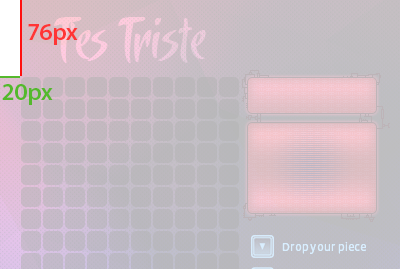
\includegraphics[scale=0.5]{img/decalage.png}
\end{center}

\subsubsection{Fonctions à implémenter}

\begin{csharpcode*}{label=Plate.cs}
public class Plate
{
    public bool IsLineFull(int y)
    {
        // Renvoie vrai si la ligne numéro y est pleine (byte 1 ou 2)
    }
    
    public void EmptyLine(int y)
    {
        // Vide la ligne y et fait tomber tous les blocs
        // au dessus de cette ligne d'une case
    }
}
\end{csharpcode*}

\subsection{Pièce}

\subsubsection{Implémentation}

On peut considérer qu'une pièce est un ensemble de 3 blocs. Chaque bloc a des
coordonnées qui lui sont propres sur la map, soit un couple $(x,y)$. \\

Pour plus de clarté, on va déclarer une structure (si vous ne savez pas ce que
c'est, considérez que c'est comme une classe) : \\

\begin{csharpcode*}{label=Piece.cs}
public class Piece
{
    public Cell[] Cells { get; set; }

    public struct Cell
    {
        public byte X { get; set; }
        public byte Y { get; set; }

        public Cell(byte x, byte y)
        {
            X = x;
            Y = y;
        }
    }
}
\end{csharpcode*}

\subsubsection{Génération aléatoire}
\begingroup
    On veut qu'à la création de la pièce, lui soit affectée une forme aléatoire.
    L'une de celles-ci : \\

    \begin{center}
        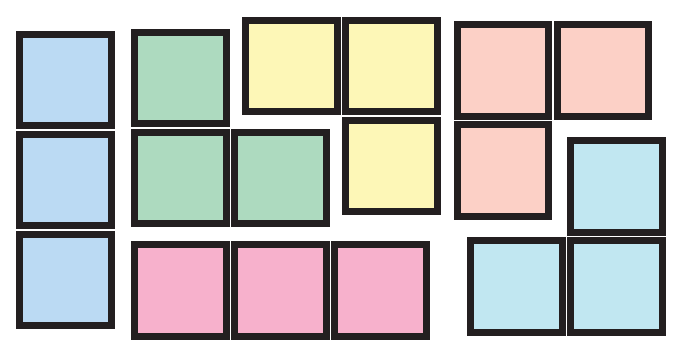
\includegraphics[scale=0.5]{img/pieces.eps}
    \end{center}
\endgroup

Et on sait que cette pièce possède 3 blocs qui ont chacun des coordonnées sur
le plateau de jeu. Vous Connaissez les coordonnées du haut du plateau de jeu.
À vous de jouer. \\

Vous devriez randomizer la pièce dans le constructeur, étant donné qu'on veut
qu'à chaque création d'une pièce, elle soit aléatoire. \\

\begin{csharpcode}
Random random = new Random();
random.Next(6); // renvoie un entier compris entre 0 et 5 (compris)
\end{csharpcode}

\subsubsection{Déplacement}

Pour pouvoir se déplacer, la pièce a besoin de savoir sur quel plateau de jeu
elle est. On va donc lui rajouter le plateau en attribut. On donnera une valeur
à cet attribut au moment de la création de la pièce, dans le constructeur donc : \\

\begin{csharpcode*}{label=Piece.cs}
public class Piece
{
    private Plate _plate;

    public Piece(Plate plate)
    {
        _plate = plate;
    }
}
\end{csharpcode*}

Pour déplacer la pièce on va :
\begin{itemize}
    \item d'abord l'enlever du plateau (mettre les bytes de ses cases à 0)
    \item calculer les nouvelles coordonnées de ses cases
    \item la remettre sur le plateau (passer les bytes de ses cases à 1)
\end{itemize}

Implémentez donc : \\

\begin{csharpcode*}{label=Piece.cs}
public class Piece
{
    // Met les bytes des cases de la pièce à 0 sur le plateau
    public void Clear(){}

    // Met les bytes des cases de la pièce à 2 sur le plateau
    public void Print(){}
}
\end{csharpcode*}

Clear() est appelée avant chaque déplacement, Print() juste après. \\

Elles seront appelées dans les fonctions : \\

\begin{csharpcode*}{label=Piece.cs}
public class Piece
{
    ...

    public void MoveDown(){}

    public void MoveLeft(){}

    public void MoveRight(){}

    ...
}
\end{csharpcode*}

\vspace{0.2cm}

Ces fonctions déplacent la pièce dans chaque direction (sauf vers le haut)
\textbf{uniquement} si il est possible pour elle de bouger (il faut vérifier
que cette condition est vérifiée avant de Clear() la pièce et de la déplacer). \\

Lorsqu'une pièce ne peut plus descendre, elle est bloquée (rappelons que dans un tétris la pièce
descend constamment). \\

Implémentez donc les fonctions suivantes : \\

\begin{csharpcode*}{label=Piece.cs}
public class Piece
{
    ...

    // Vérifie qu'une pièce peut descendre d'une case
    public bool CanGoDown();

    // Passe les bytes des cases de la pièce à 1 sur le plateau de jeu
    public void Block();

    ...
}
\end{csharpcode*}

\subsection{Boucle de jeu principale}

Première chose à faire, ajouter à notre jeu les bons attributs :

\begin{csharpcode*}{label=Game1.cs}
public class Game1
{
    ...

    // On va avoir besoin de compter le nombre de fois qu'on passe sur la
    // fonction Update(), pour bouger la pièce automatiquement vers le bas
    // à partir d'un certain nombre de fois.
    private int _timer;

    // On va mettre notre plateau de jeu ici :)
    private Plate _plate;

    // Ainsi que notre pièce actuellement en mouvement
    private Piece _currentPiece;

    // Une énumération des états possibles que peut prendre notre jeu
    // Si vous avez du mal avec les enum, mettez un booléen IsRunning
    enum GameState { Running, GameOver }

    private GameState _gameState;

    ...
}
\end{csharpcode*}

\subsubsection{Initialisation du jeu}

\begin{csharpcode*}{label=Game1.cs}
public class Game1
{
    ...

    protected override void Initialize()
    {
        // TODO: Créer un nouveau plateau de jeu (Plate) et le mettre dans _plate
        
        // TODO: Créer une nouvelle pièce
        
        // Passe l'état du jeu en 'Running'
        _gameState = GameState.Running;

        // Le code qui suit change la taille de la fenêtre :
        graphics.PreferredBackBufferWidth = 400;
        graphics.PreferredBackBufferHeight = 580;
        graphics.ApplyChanges();

        // TODO: Récupérer l'état courant du clavier dans _pKs et _cKs

        base.Initialize();
    }

    ...
}
\end{csharpcode*}

\subsubsection{Détection du GameOver}

Implémenter la fonction qui détecte si la partie est finie. \\

\begin{csharpcode*}{label=Game1.cs}
public class Game1
{
    ...

    private bool IsGameOver()
    {
        // TODO: vérifier les bytes de la map pour savoir si la partie est
        //       terminée
    }
    
    ...
}
\end{csharpcode*}

\subsubsection{Update()}

Notre première boucle de jeu. Voilà ce qu'il faut faire dedans : \\

\begin{csharpcode*}{label=Game1.cs}
public class Game1
{
    ...

    protected override void Update(GameTime gameTime)
    {
        // TODO: vérifier que l'état de la partie n'est pas à GameOver
        //       Si c'est le cas, retourner (return;)

        // Vérifier que le joueur n'appuie pas sur 'flèche gauche' ou
        // 'flèche droite'. Si c'est le cas, on bouge la pièce en conséquence.

        // TODO: Incrémenter le _timer

        // TODO: Si (_timer == 20) et que la pièce peut descendre vers le bas,
        //          on la descend.
        //       Sinon, on bloque la pièce, on vérifie qu'il n'y a pas de ligne
        //          pleine. Si c'est le cas on les explose (récursivement, il peut
        //          y avoir plusieurs lignes pleine en même temps (max 3)
        //       Et on vérifie que la partie n'est pas terminée. Si c'est le cas
        //          on passe _gameState à GameState.GameOver
    }

    ...
}
\end{csharpcode*}

\subsubsection{Draw()}

\begin{csharpcode*}{label=Game1.cs}
public class Game1
{
    ...

    protected override void Draw(GameTime gameTime)
    {
        spriteBatch.Begin(); // Rajoutez cette ligne

        // TODO: Afficher la texture GameBackground

        // TODO: Afficher le plateau de jeu

        // TODO: Si l'état du jeu est GameOver, on affiche la texture
        //       GameOver par dessus le tout

        spriteBatch.End(); // Rajoutez cette ligne

        base.Draw(gameTime);
    }

    ...
}    
\end{csharpcode*}

\section{Bonus}

Si vous êtes vraiment des malades et que vous avez tout fait, vous pouvez vous
amuser à implémenter ces quelques fonctionnalités supplémentaires :

\begin{enumerate}
    \item Rajout d'un état de jeu 'Pause'
    \item Drop (la pièce tombe le plus bas possible et se bloque)
    \item Scoring
        \begin{enumerate}
            \item Calcul du score
            \item Affichage du score (SpriteFont XNA)
        \end{enumerate}
    \item Piece holding (le joueur garde une pièce en mémoire)
\end{enumerate}

\section{Conclusion}

\emph{In GConfs You Trust.}

%

\end{document}

